\documentclass{article}
\usepackage{graphicx} % Required for inserting images
\graphicspath{ {./images/} }
\usepackage{hyperref} % for hyperlinks
\usepackage{microtype}
\usepackage{subfigure}
\usepackage{booktabs} % for professional tables
\usepackage{amsmath}
\usepackage{stfloats}
\usepackage{authblk}
\usepackage[square,numbers]{natbib}
\bibliographystyle{unsrtnat} % or 'plainnat' if you prefer


% Attempt to make hyperref and algorithmic work together better:
\newcommand{\theHalgorithm}{\arabic{algorithm}}

\usepackage[margin=1in]{geometry}

\title{\textbf{“It looks like you’re working out.”\\Using Machine Learning Classification Techniques to Predict Physical Stress}}

\author{
\begin{tabular}{c}
Eva Schwartz \\
DATS 4001: Data Science Capstone \\
Department of Data Science \\
George Washington University \\
\texttt{eschwartz25@gwu.edu}
\end{tabular}
}

\date{} % no date

\begin{document}

\maketitle

\twocolumn

\begin{abstract}
Predicting physical stress is one of the most important factors in the development of fitness wearables. In this paper, I present a research project aimed at predicting physical stress using wearable technology data and machine learning classification techniques. A traditional Logistic Regression model, a Random Forest, an XGBoost classifier, a Histogram Gradient Boosting classification, and a Multi-Layer Perceptron model were used in the research. Specificity and negative predictive value was used to compare models, with Random Forest and XGBoost emerging as very strong models for this task. The most significant feature in predicting physical stress was temperature. The findings from this research could be applied to other health-focused fields or issues, such as classification of rare disease. Given the subject demographic of this dataset was majority male, repeating this comparison research on a demographic with even gender proportions would be valuable, though the lack of female inclusion in health datasets could pose an issue in this future research step.
\end{abstract}

\section{Introduction}
If you use a wearable fitness watch, you might have looked down and seen a message like the one pictured below prompting you to start a workout when you are actually not working out. 
\begin{center}
    
\includegraphics[scale = .28]{images/Apple_Watch_Workput_Detection_banner-800x457.jpeg}
    \cite{appleWatch}
\end{center}
This incorrect notification is a product of predicting physical stress, and sometimes even highly developed models and products get predictions wrong. This is not a huge surprise though, as the Center for Disease Control recommends 150 minutes of moderate-intensity physical activity a week, and put into the perspective of a full week, this recommendation is only 1.4\% of an average adult’s week, representing a clear imbalance. While it may be annoying to recieve an additional notification prompting you to start a workout, fine tuning and selecting models to deliver and predict physical stress is a valuable part of wearable fitness development. My strong interest in endurance activities, predicting physical stress, and machine learning prompted me to investigate this issue for my Data Science Capstone project. Through this project,I hope to investigate predicting physical stress using wearable technology data and machine learning classification techniques. 


\subsection{Overview of Machine Learning Model Comparison}

Classifying imbalanced data is a struggle across domains and fields. The performance of machine learning classifiers is impacted by the ratio of the majority class to the minority class. In imbalanced datasets, this can cause classifiers to be biased towards the majority class.

When classifying imbalanced data, model evaluation metrics are vital in understanding which models are the strongest for predicting classification groups. To compare, metrics like accuracy, precision, and recall are used.

To calculate these metrics, a confusion matrix is necessary. Confusion matrices are used in binary classification and are predicated on the idea that the majority class is designated as the negative class and the minority class is designated as the positive class. For binary classification, the layout of the confusion matrix can be seen in Figure 1. 

\begin{center}
    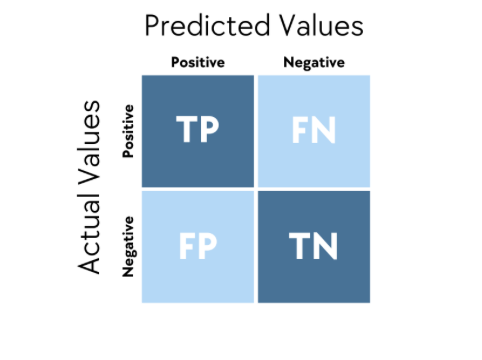
\includegraphics[scale = .75]{images/CM.png}
\end{center}

Metrics like accuracy, recall, precision, specificity, and negative predictive value can be derived from the results of confusion matrices. For this research, the ‘positive’ majority class is the non-active, resting state, and the ‘negative’ minority class is the active, physical stress state. 

Accuracy is formulated by the proportion of all classifications that were correctly classified, positive or negative, over the total classification count. It is defined as the following: 

\begin{center}
    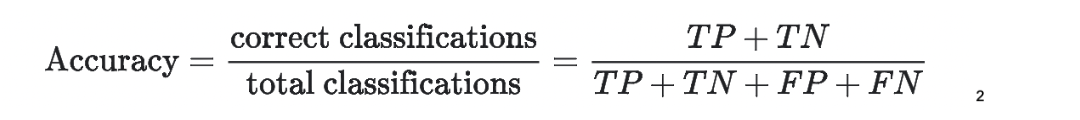
\includegraphics[scale=.45]{images/ACCURACY.png}
\end{center}

Accuracy is useful, but in the case of imbalanced classification, a false positive or false negative can be more costly. In the case of predicting physical stress, a false negative – predicting no physical stress when physical stress is present – can be more costly than a false positive – predicting physical activity stress when physical stress is not present – therefore, other evaluation metrics can be more helpful for imbalanced data. 

Recall is the true positive rate, and is measured as the proportion of actual positives that were correctly classified as positives. It is also known as the true positive rate. It is defined as the following: 
\begin{center}
    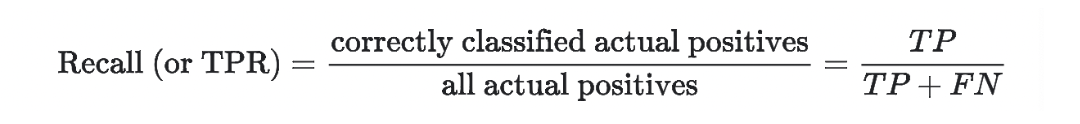
\includegraphics[scale=.45]{images/RECALL.png}
\end{center}

In imbalanced data, recall is generally can be more helpful than accuracy because it focuses on evaluating a model’s ability to predict positive classes, thereby reducing the possibility of a false negative. For the purpose of this imbalanced data though, recall is less helpful given its focus on predicting positive classes as the minority class for this data is the negative class. 

Precision is another model evaluation metric that uses the proportion of correctly classified actual positives over all points classified as positive to find actual positive values. It is not as useful for imbalanced data in general, as actual positives in most imbalanced datasets represent a very small percentage of total data, therefore, precision is less meaningful and useful as an evaluation metric in imbalanced data. The formula for deriving precision is as follows:

\begin{center}
    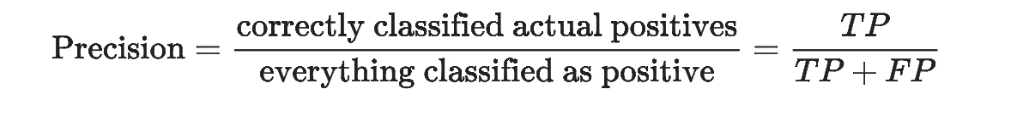
\includegraphics[scale=.45]{images/Precision.png}
\end{center}

Precision and recall generally have an inverse relationship, where improving precision or recall worsens the other. This is because precision improves as false positives decrease, while recall improves when false negatives decrease. 

Specificity is a metric focused on identifying how well a model identifies actual negative classes. It is also called the true negative rate. Specificity is particularly strong for this imbalanced dataset, as the class this research is focused on predicting is the negative class. Specificity is therefore a stronger evaluative metric than accuracy or recall given its focus on predicting the negative class, which is physical stress in this research. The formula below demonstrates how specificity is derived. 

\begin{center}
    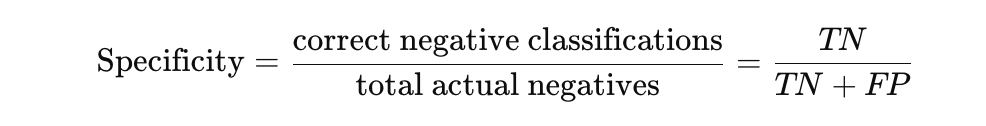
\includegraphics[scale = .45]{images/specificity.png}
\end{center}

Negative predictive value, or NPV, is another metric that is vital for this research. It derives the accuracy of negative predictions by models, operating as the inverse of precision which analyzes the positive predictions of models. NPV is vital in comparing the models used in this research as the goal of this project is to predict the negative class - the active physical state. The formula for deriving NPV is below. 

\begin{center}
    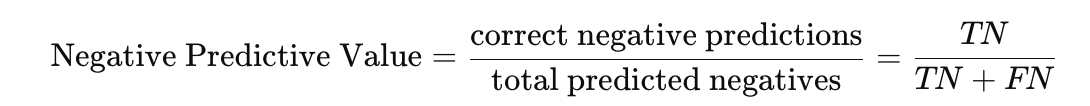
\includegraphics[scale = .40]{images/NPV.png}
\end{center}

The receiver-operating characteristic curve, or ROC curve, serves as a visual representation of model performance across various thresholds of model training. The ROC curve is drawn by calculating the true positive rate and the false positive rate at every possible threshold, then graphing the true positive rate over the false positive rate. The higher the true positive rate and the lower the false positive rate, the better, so in the ROC curve, models that are centered more in the top-left side are better.

The area under the ROC curve, denoted as AUC, represents the “probability that the model, if given a randomly chosen positive and negative example, will rank the positive higher than the negative.” ~\cite{googleML} When data is balanced, AUC is a useful measure for comparing performance across models, but in this imbalanced dataset, true negatives are more valuable than true positives, therefore ROC AUC is a less valuable metric. 

Precision-recall AUC curves can be strong for evaluating model performance in imbalanced datasets. PR AUC uses a precision-recall curve by plotting precision over recall, with higher y-axis values indicating stronger model performance. The area under the precision-recall curve indicates the average of precision scores calculated for each recall threshold, and once recall starts to drastically fall and lower the y-axis values in this curve, this is a strong indication that the model has passed its optimal precision-recall threshold. Though PR AUC focuses on plotting precision against recall and therefore centers on the majority, positive class, this metric can still be valuable in comparing models for this research. This is because if a model has a higher PR AUC score it can indicate that it is correctly identifying the rare negative cases, is avoiding false negatives, and is avoiding false positives. 

\section{Related Work}

In broader classification tasks with extremely imbalanced data, the detection of credit card fraud is a commonly cited example. One team working on credit card fraud detection used a dataset where their positive class accounted for 0.2\% of their dataset.~\cite{dalpozz} This is an example of extreme class imbalance, with extreme class imbalance defined as any dataset where the minority class accounts for 1\% or less of the dataset.~\cite{googleML} They noted that when wanting to classify the most suspicious transactions, they recommend assigning larger class weights to the fraudulent transactions they are looking to predict, where class weights define the relative importance of each class in the training process .~\cite {MATLABHelp}

A similar study focusing on detecting fraudulent credit card activity implemented classification techniques on a similarly imbalanced dataset, with 0.4\% of values belonging to the minority class of fraudulent transactions.~\cite{AFRIYIE2023100163}  This study compared a decision tree, random forest, and logistic regression model. Prior to running their models, they balanced the data using an under-sampling technique. Under-sampling can be used to balance datasets by bringing the value counts of the majority class down to the same value counts of the minority class. While this is a powerful way to balance datasets, experiments run the risk of discarding valuable data points that could form a richer, more robust model. Nonetheless, they found that Random Forest had the highest accuracy, recall, and precision with values of 96\%, 97\%, and 9\%, respectively. 

Arriving at the health and human biology field, the prediction of physical stress suffers from imbalanced data as well. Lazarou and Exarchos discuss emotional and physical stress in their article, noting that wearable sensors offer strong data collection techniques for predicting physical stress by providing real-time feedback on biomarkers.~\cite{Lazarou2024} They discuss the role of the sympathetic nervous system (SNS) in detecting stress. The SNS is activated when the body detects perceived threats, which triggers the release of norepinephrine and epinephrine, causing tandem biological responses including heightened heart rate, increased blood flow to muscles, increased alertness, and more. 

In their article, Lazarou and Exarchos note how electrocardiogram activity, which measures the heartbeat, and electrodermal activity, which is a measure of the electrical conductance of the skin and is measured as changes due to sweat secretion, are common biophysical and biochemical parameters of stress. These indicators serve as mental and physical indicators of stress and are investigated as variables in the following experiments. 

\section{Methods}
The following section will outline the dataset used and data preparation steps while discussing the sensor-fused variables and the motivation behind including these variables. 

\subsection{Dataset}
The dataset used is publicly available from PhysioNet and provides non-EEG physiological signals with features including electrodermal activity, temperature, acceleration, race, heart rate, and arterial oxygen level. The data were collected using noninvasive wrist-worn Empatica biosensors. The dataset consisted of 20 subjects, with 30\% of the sample as female subjects, and a mean overall age of 26.05 years. The dataset consists of 7 stages for the given subjects. Stage 1 is a five-minute period of relaxation. Stage 2 is a five-minute physical stress period, in which subjects were instructed to “stand for one minute, walk on a treadmill at one mile per hour for two minutes, then walk/jog on the treadmill at three miles per hour for two minutes.”~\cite{Birjandtalab2016} Stage 3 was another five-minute relaxation stage, then stage 4 consisted of cognitive stress for the subjects. Stage 5 was another relaxation stage, which was followed by stage 6 with a five-minute emotional stress stage. Finally, stage 7 consisted of 5 minutes of relaxation. 

\subsection{Data Processing}


The first stage of data preprocessing consisted of syncing the timing of each subject together. The data frame with heart rate and respiratory rate was measured in 1-second intervals for each subject, while the data frame for each subject's acceleration rate, body temperature, and electrodermal activity was measured in 0.125-second intervals. To synchronize these data frames, each value for the respiratory rate and heart rate data was multiplied by 8 to match the other data frame, without losing any data. Next, according to the delineation of the given stage by the authors of the data set, a binary variable was added to indicate physiological stress. 

After checking for missing data, of which there were none, outlier detection was performed. To find outliers, an isolated forest model was used. The isolation forest focuses on detecting anomalies by finding how far a given data point is from the rest of the data. It introduces binary trees, then forms partitions in the binary trees by randomly selecting features, then forming a random split value for the feature. This process is continued until the max depth of the trees is one, that is, until the partitioning process separates a given data point from the rest of the samples. While this step was valuable in my data processing, the primary intention of performing this outlier detection was to explore the data. While each subject’s outliers were detected individually to account for variations across subjects, removing outliers would minimize the dataset. Furthermore, detecting outliers in physiological data invites an inherent degree of variability, therefore, this step was focused more on exploration. 


\section{Feature Extraction}

To enhance the strength of my dataset, I next performed feature extraction and sensor fusion on some of my variables. I started by forming an acceleration magnitude variable by applying the following formula to the respective acceleration values on the x-axis, y-axis, and z-axis: 


\begin{equation}
    \|\vec{a}\| = \sqrt{a_x^2 + a_y^2 + a_z^2}
    \label{eq:vector_magnitude}
\end{equation}

Forming this variable enhances the dataset as it forms a whole measure of acceleration, bringing further depth and information to the degree of physical activity a given subject was undergoing.~\cite{Arif2014} Acceleration magnitude can aid in understanding the intensity of physical activity, while also supporting identification of changes in motion. 

Next, I investigated the ratio of a given subject’s heart rate to their acceleration magnitude. This engineered feature adds to the dataset by aiding in indicating the intensity of a subject’s physical activity. Biosignal relationships imply that as a subject’s acceleration magnitude increases, their heart rate increases as well. The final feature engineered variable is a ratio of body temperature to electrodermal activity. Body temperature is a result of the body’s thermoregulatory processes, which are neurological and controlled by the hypothalamus. Electrodermal activity is controlled by the sympathetic nervous system, and while the relationship between the biosignals that make up EDA is very complex, EDA is influenced by body temperature, and therefore, a ratio of these variables would further enhance my dataset. 

\section{Experiments}

The baselines for class distribution in similar extreme imbalanced dataset machine learning research indicate that extreme class imbalance is present if less than 1\% or less of the data belongs to the minority class. The dataset used in this research consists of 99.45\% negative samples and .54\% positive samples, indicating that the dataset is extremely imbalanced. To combat extreme class imbalance, there are a couple of options. Undersampling, as mentioned above, involves removing the majority class samples.~\cite{leborgne2022fraud} This class balancing technique is strong, though it reduces the size of a given dataset, which could result in poorly fitted models. Oversampling serves as the opposite approach and artificially increases the proportion of samples from the minority class. One standard method that interpolates samples from the minority class is the Synthetic Minority Oversampling Technique (SMOTE). SMOTE techniques can be extended to hybrid resampling techniques, in which the minority class is interpolated while undersampling techniques clean up common data points that confuse the model. 

In my implementation, I chose to implement SMOTETomkek hybrid resampling to balance my dataset. This resampling technique uses traditional SMOTE resampling to augment the minority class while simultaneously using Tomek undersampling.~\cite{tomek} Tomek Link undersampling is a modification of condensed nearest neighbor techniques, and removes samples of the majority class by finding the nearest neighbor for each data point. If the nearest neighbors belong to different classes and are nearest neighbors, the data points form a Tomek Link, and the majority class point is removed to emphasize the decision boundary of the data. 

\subsection{Implementation}

Before completing the aforementioned resampling techniques, I split the data for cross-validation. Splitting data ahead of resampling is vital, as it minimizes the potential for data leakage across training and testing sets. 

To ensure robust cross-validation techniques, I implemented a Stratified K-Fold method using 3 inner folds for tuning hyperparameters, then 5 outer folds for training and testing models. I wanted to ensure I fully accounted for the unbalanced distribution of my data. Using stratified k-fold cross-validation techniques ensures that data distribution is maintained across folds, ensuring robust data preparation.~\cite{Prusty2022} Furthermore, standard k-fold cross-validation would not guarantee representation of the minority class, which is vital in training my models. With stratified k-fold cross validation, samples are ordered by class, then within each respective class, they are divided into the given K sets to ensure classes are represented across folds. The stratified folds are then formed by adding the first stratum from each class to combine these as the first fold, then continuing in this manner for each fold. Then one fold serves as the test set, with the remaining K-1 folds used for training. The image below demonstrates how the class distributions are sampled. 

\begin{center}
    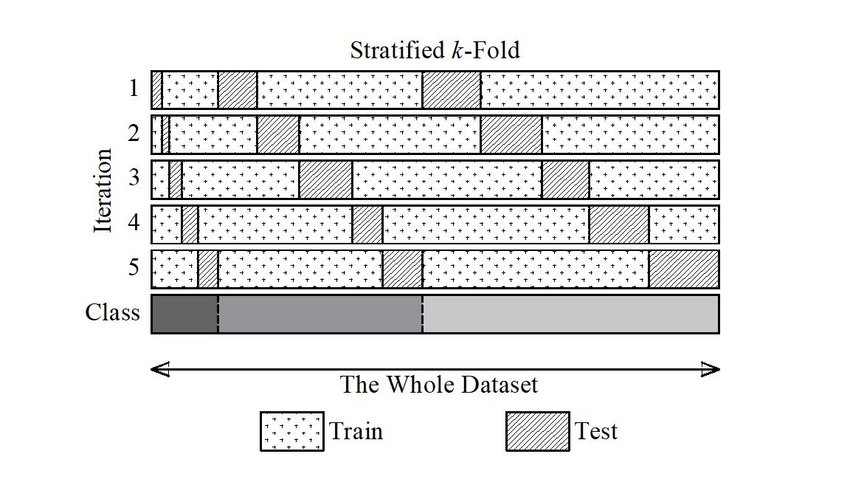
\includegraphics[scale = .60]{images/skf.jpeg}
~\cite{SKFIMAGE}
\end{center}

For the initial run of each model, five strata were used. Then, to test the performance of the model selection and model parameters, three strata were used. Following the splitting of data but before the data was fed into models, the data was scaled using the MinMaxScaler. The decision to use MinMaxScaler over other scaling models, such as StandardScaler, was due to MinMax’s implementation of proportional transformations within the range [0,1].~\cite{scalercomparison} StandardScaler transforms values in a given column to have a mean of 0 and a standard deviation of 1, but assumes that data is normally distributed and allows negative values. These assumptions are not satisfied due to the nature of the data used, following a non-normal distribution and inability to have negative values for included biosignals. Furthermore, MinMaxScaler is recommended when upper and lower boundaries are known from domain knowledge, as is the case for most of the biosignals in this dataset. Therefore, the MinMaxScaler emerged as a strong standardization tool. 

In implementing my models, I used RandomizedSearchCV to fit models across parameter settings while efficiently comparing models given limited computational resources. The models I compared in my research are a traditional Logistic Regression model, a Random Forest classifier, an XGBoost classifier, Histogram Gradient Boosting classification, and a Multi-Layer Perceptron model. 

Logistic regression is a very traditional supervised machine learning algorithm that utilizes a sigmoid activation function to model the relationship between independent variables and the probability of a binary outcome. Sigmoid functions convert real values of predicted values into an S-shaped curve with a binary value between 0 and 1. Including this model serves as a baseline for model comparison, given that logistic regression is the simplest classification model. 

Random forest models use an ensemble of decision trees trained with bagging methods. They introduce randomness in searching for the best features in growing trees to avoid computationally intensive methods of feature importance. ~\cite{MachineLearningI} The randomness allows for further tree diversity, while giving higher bias with lower variance to form a better overall model. This is a basic, commonly used decision tree model in machine learning, and serves as a strong baseline above logistic regression models. 

Histogram Gradient Boosting is also a member of the decision tree family, and it accelerates the random forest model by discretizing continuous variables in datasets to unique values to train models around these binned variables, resembling histogram plots. Boosting adds tree models to decision tree classifiers and each additional model attempts to correct the mistakes of the previously added models to “boost” the output of the final model.~\cite{MachineLearningI} Histogram Gradient Boosting utilizes boosting and discretization to optimize decision tree classification tasks, allowing for strong model performance, especially for larger datasets. 

XGBoost, which stands for Extreme Gradient Boosting, uses parallel tree creation to create multiple decision trees, then uses boosting, like histogram gradient boosting. In this approach, random forest bagging works to minimize variance and overfitting in models, while boosting minimizes bias and underfitting. XGBoost optimizes for computational efficiency and model performance by building trees in parallel, learning from the mistakes of prior trees, then delivering a very strong model within the tree-based models family. The architecture of XGBoost models can be seen below: 

\begin{center}
    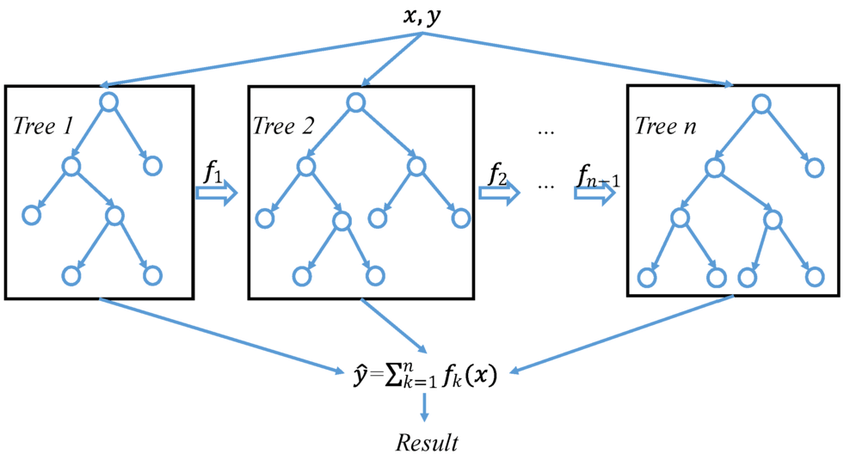
\includegraphics[scale = .25]{images/XGBOOST.png}
    ~\cite{xgboost}
\end{center}

Histogram-based gradient boosting and XGBoost are very similar, but differ in their input variables. Comparing their performance was something I was interested in examining to understand the role of discretization on model performance. 

I implemented a Multi-Layer Perceptron Classifier as well. MLP classifiers use an input layer, then multiple hidden layers, then an output layer to predict classification tasks. The hidden layers require an activation function to pass results, and my models used ReLU (Rectified Linear Unit) activation, allowing for results to pass through layer by layer to generate class predictions. This activation function avoids the vanishing gradient issue that plagues neural networks, whereby machine learning models that use backward propagation have increasingly small updated weights. This issue can stall the learning process and prevent models from learning patterns. The MLP classifier with ReLU activation avoids this as it uses forward propagation to continuously feed inputs through hidden layers. An example of the architecture for these models can be seen below. 

\begin{center}
    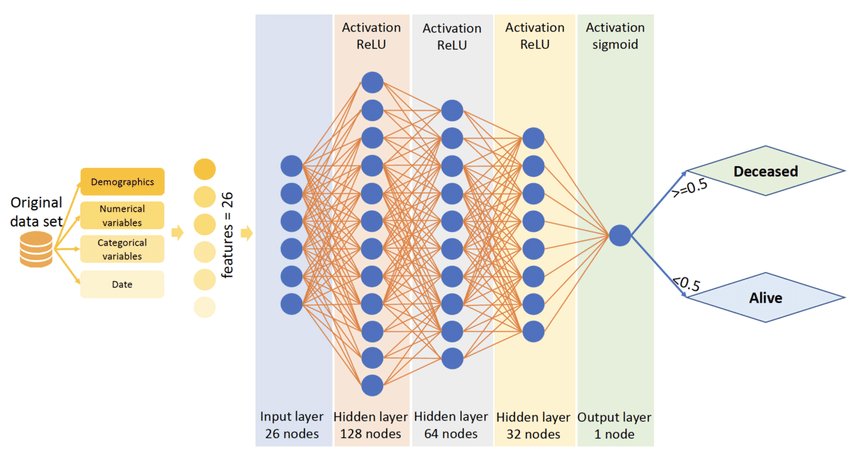
\includegraphics[scale = .25]{images/RELU.png}
    ~\cite{RELUImage}
\end{center}

While single and multi-layer perceptrons are strong models, they were created based on human neural networks, and therefore, these systems are plagued by the “black box issue,” in which there is a lack of information regarding how MLP models arrive at their class predictions. They can reflect hidden biases, similarly to human thought patterns, which introduces weakness into the explainability of these models. Therefore, though neural networks provide strong modeling outcomes, their construction should be taken into consideration, especially in a human biology setting. 

\section{Results}
After tuning hyperparameters on three inner stratified k-folds, the final models and hyperparameters were evaluated on the five outer stratified k-folds. This allowed for 80\% of the training data to be used in each fold, while ensuring that the original class distribution was maintained. 

\subsection{Results of Models}

After using RandomizedSearchCV() to find the best-performing hyperparameter, the final models delivered the results featured in the model summary table at the top of the following page. Additionally, hyperparameters for best performing models of each model class can be found in the Appendix.

\begin{figure*}[t]
    \centering
    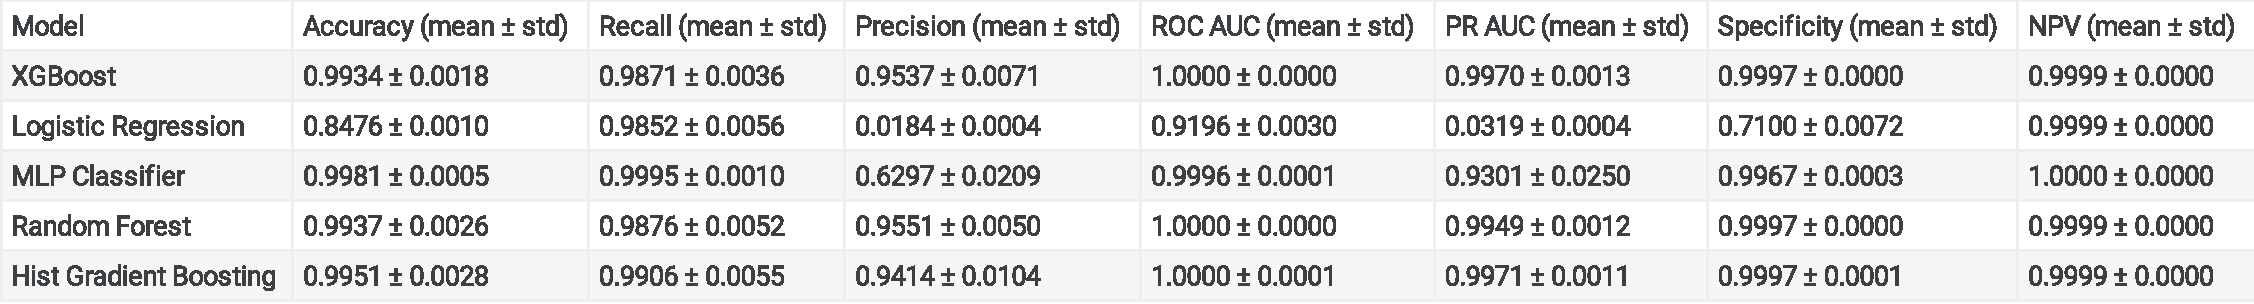
\includegraphics[scale = .4]{images/summary chart.pdf}
    \caption{Summary of model evaluation metrics for best performing respective models}
\end{figure*}

As discussed in Section 1.1: Overview of Machine Learning Model Comparison, specificity and NPV are key in comparing classification models for imbalanced datasets where the minority class is the negative class. XGBoost, Random Forest, and Histogram Gradient Boosting all have the highest specificity for the best performing models of each model class. All models had strong negative predictive value, with the Multi-layer Perceptron having the highest, though the difference between each model's NPV is very small. Logistic Regression's simplicity can be seen in the model metrics, which is to be expected given the simplicity of this model.

Though the PR AUC curve is best for imbalanced data where the positive class is the minority class, it can still be valuable in this data as a high PR AUC score indicates that a model is minimizing false predictions of both negative and positive classes. Histogram Gradient Boosting was the best performing model regarding PR AUC, with comparison plots featured below. 

\begin{center}
    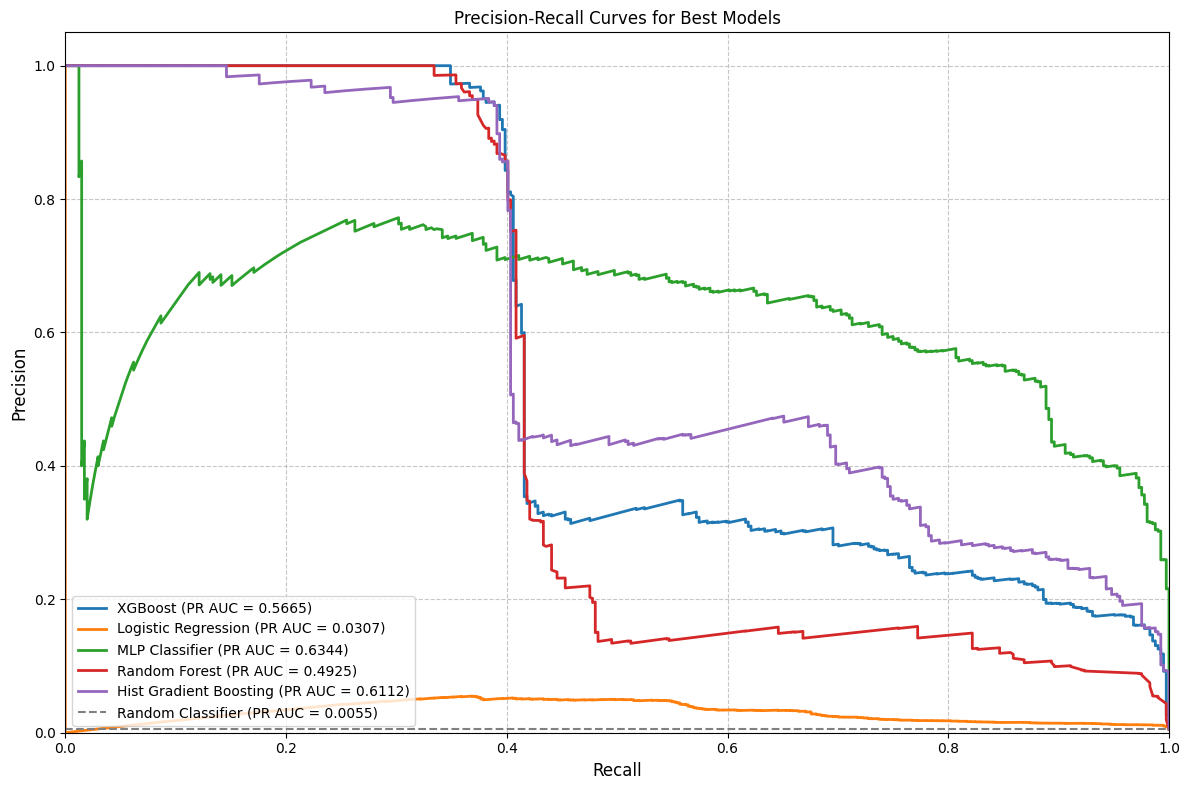
\includegraphics[scale = .25]{images/PR curves.png}
\end{center}

Given that the tradeoff between precision and recall is valuable in classifying imbalanced datasets, no matter the majority class, the Histogram Gradient Boosting model had strong performance in this category. The random classifier with the lowest PR AUC serves to demonstrate the precision-recall tradeoff for an untrained model, indicating that Logistic Regression did only slightly better than this randomly classifying model without hyperparameters to train.

As discussed in Section 1.1: Overview of Machine Learning Model Comparison, confusion matrices serve as the baseline for calculating the aforementioned metrics. Below are the confusion matrices for the model iterations in the final, fifth fold of data:

\begin{center}
    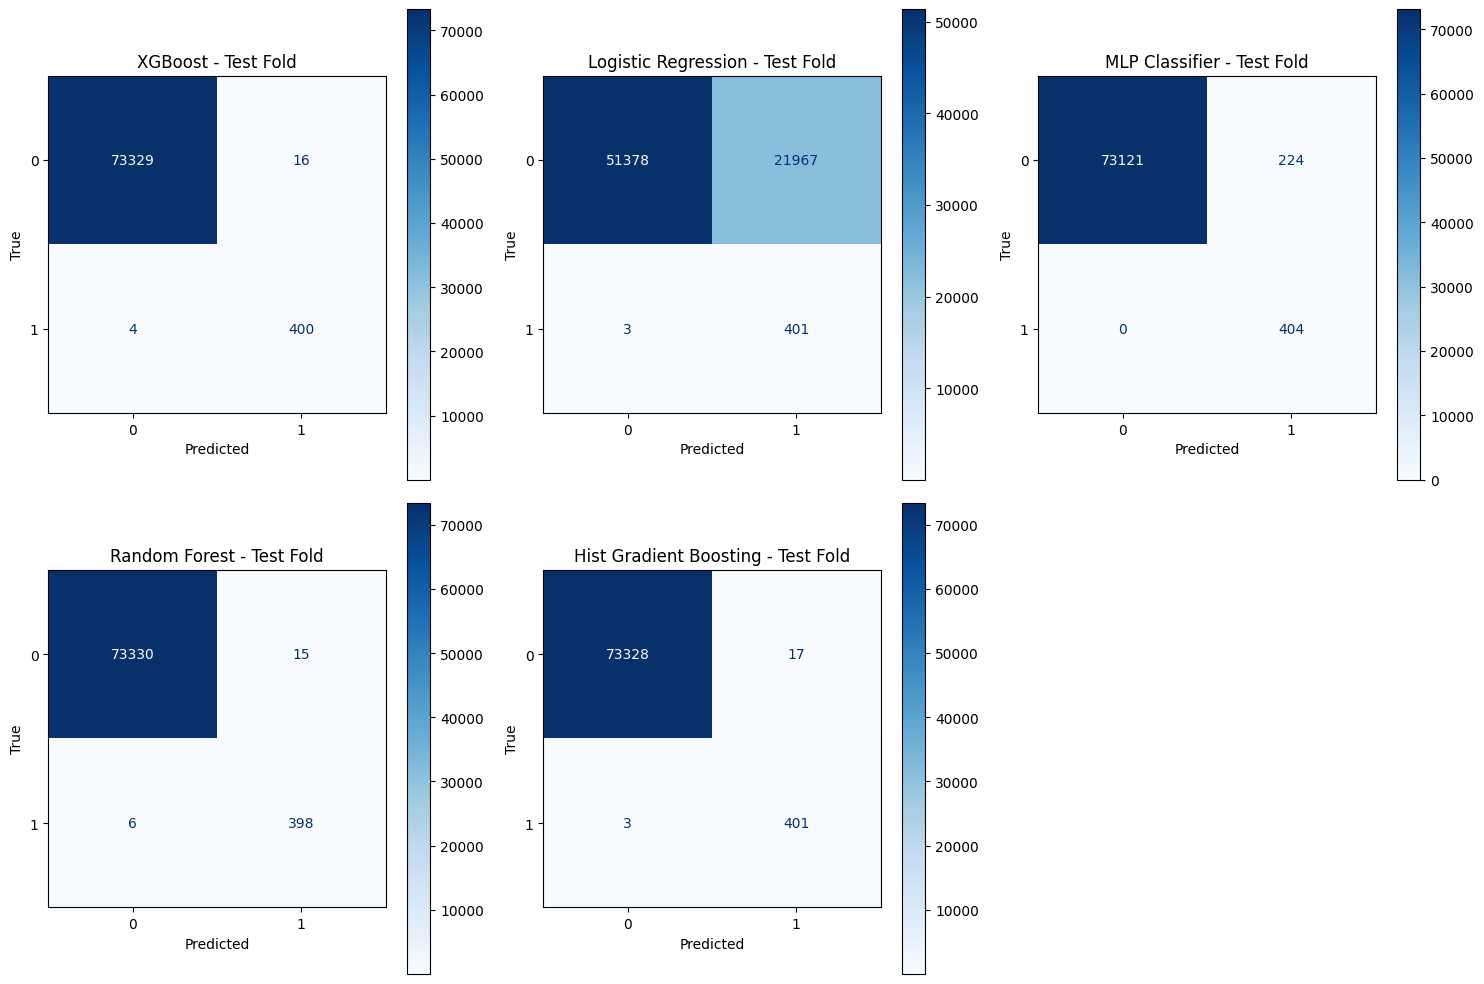
\includegraphics[scale = .20]{images/confusion matrices.png}
\end{center}

XGBoost, Random Forest, and Histogram Gradient Boosting all demonstrate their strength in predicting physical stress, both negative and positive cases. The simplest classification model, Logistic Regression, struggles to correctly classify true positives, which in this context represent times of rest. This indicates that a simpler model may not be as adept at predicting extreme imbalanced datasets, given issues in predicting the majority class. 

Examining the feature importance of some of these models allows extension beyond comparing the strength of various machine learning models for classifying physical stress. Using the feature importance of XGBoost in the best-performing XGBoost model, temperature emerged as a strong feature in predicting physical stress. Full feature importance can be seen below for XGBoost: 

\begin{center}
    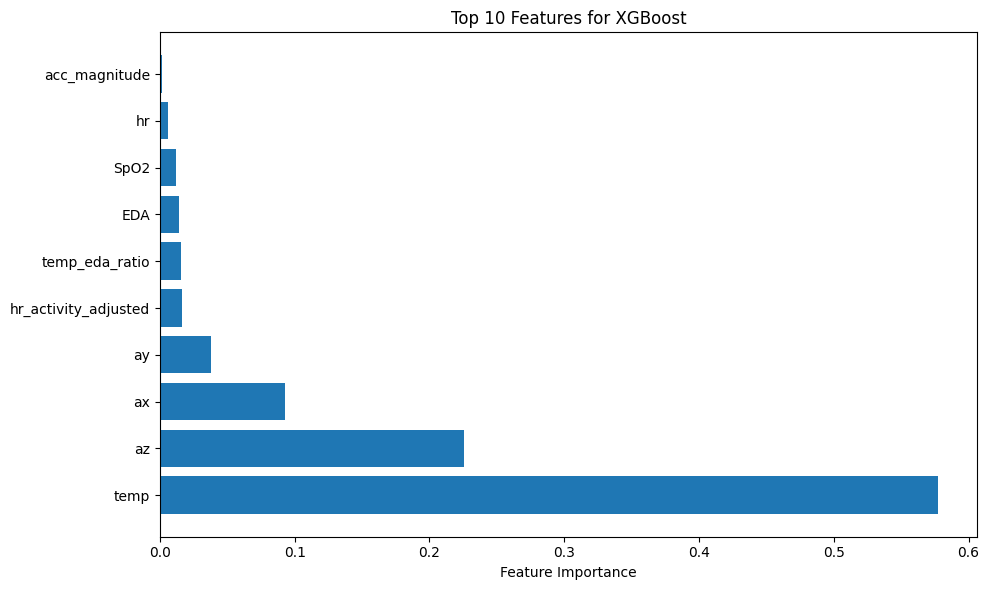
\includegraphics[scale = .25]{images/XGBOOST FI.png}
\end{center}

These results could indicate to manufacturers of fitness wearables that finely calibrating and developing body temperature sensors is vital in predicting physical stress. Additionally, the z-axis acceleration feature was an additional strong variable. This could also signal to wearables developers that fine-tuning forward and backward detection in acceleration sensors is significant in correctly predicting physical stress. 

Random Forest's feature importance demonstrates similar findings. The below feature importance indicates that temperature may not be as important to this model as XGBoost. Like XGBoost, z-axis acceleration follows in importance, then electrodermal activity emerges as an additional significant feature. As with temperature and z-axis calibration, ensuring sensors are calibrated to correctly predict and handle electrodermal activity is vital in the development of fitness wearables. 

\begin{center}
    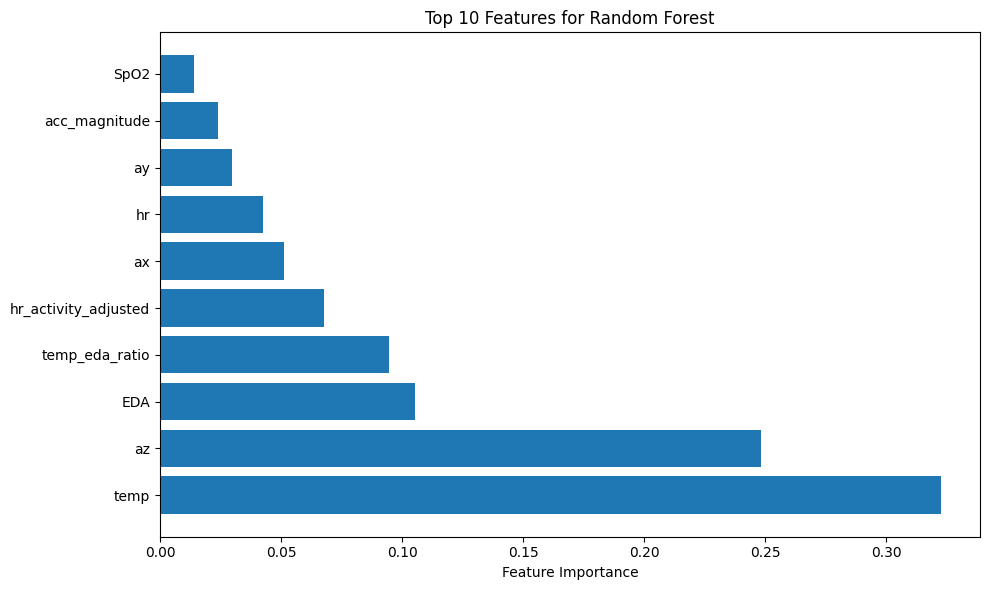
\includegraphics[scale = .25]{images/RF FI.png}
\end{center}

\subsection{Limitations}

One limitation of my research is that the dataset has more male subjects than female subjects. Therefore, though these models had strong performance their performance on a true, diverse dataset with equal representation in gender and age may change. 

Additionally, there are always inherent difficulties in predicting on extremely imbalanced datasets. As discussed in my Introduction, false positives sneak through in even the most well-developed models and products. Therefore, though my project has strong results, these findings are fully recommendations and serve to compare the models implemented in my research rather than recommend one specific model for predicting physical stress. Recommending one specific model could open up the possibility of unintended false predictions, therefore this limitation indicates that comparing models is more powerful. 

Regarding models implemented in this research, as discussed in Section 5.1: Implementation, the Multi-Layer Perceptron Model operates as a "black box," meaning that for most models there is not much information on how hidden layers arrive at their predictions given the strong inner-connectivity between the hidden layers. Therefore, though this model performs well in predicting physical stress, there is not information available on feature importance, which is a valuable metric in comparing and developing models. 

\subsection{Alternate Applications}

One alternate application for this research could be to apply the findings and model results to prediction of cybersecurity attacks or breaches. Classification of cyber attacks generally suffer from similar imbalanced data issues as predicting physical stress, therefore the model applications in this research could likely be applied to this issue as well. 

Given the health-focused development in the implementation of this research, the findings could likely be applied to broader medical fields as well. Classification and prediction of disease, for example, also generally suffers from the imbalanced data issues seen in this research. Therefore, the findings and model comparison research from this project could be applied to other health-focused fields or issues, such as classification of rare disease.

\section{Conclusion}

Multi-layer Perceptron, Random Forest, and XGBoost are all strong models for this task. While these models are strong, they are computationally intensive and not well suited for real-time physical stress classification. Therefore, implementing lighter, faster models, such as LightGBM, for classifying physical stress with online learning could be a powerful next step for this body of research. 

Temperature emerged as a very important factor in predicting physical stress across models. This finding underscores the need for developers to focus on careful calibration and development of wearables sensors to accurately predict body temperature. Given the importance of this variable in prediction and classification of physical stress, errors in this sensor could increase the likelihood of false predictions, indicating the need for careful calibration.

An interesting exploration for this research would be to compare the results of these models to those gathered from a dataset with stronger gender balance. This could allow for greater generalization of the findings from this research, due to the implementation of this research on a male-dominant dataset. While this would be a fruitful examination, the lack of female inclusion and representation in health datasets could limit this path of research. This roadblock highlights the broader issue of gender exclusion in health research, indicating the need to create more representative health technologies.

Through this project, I successfully explored my interest in physical stress and endurance sports through a data science perspective. As an active person and endurance sport athlete, understanding the role of these biosignals in predicting physical stress goes beyond my Data Science Capstone; it applies to my everyday life. 

\newpage
\appendix
\section{Hyperparameters for Best Performing Models by Fold}
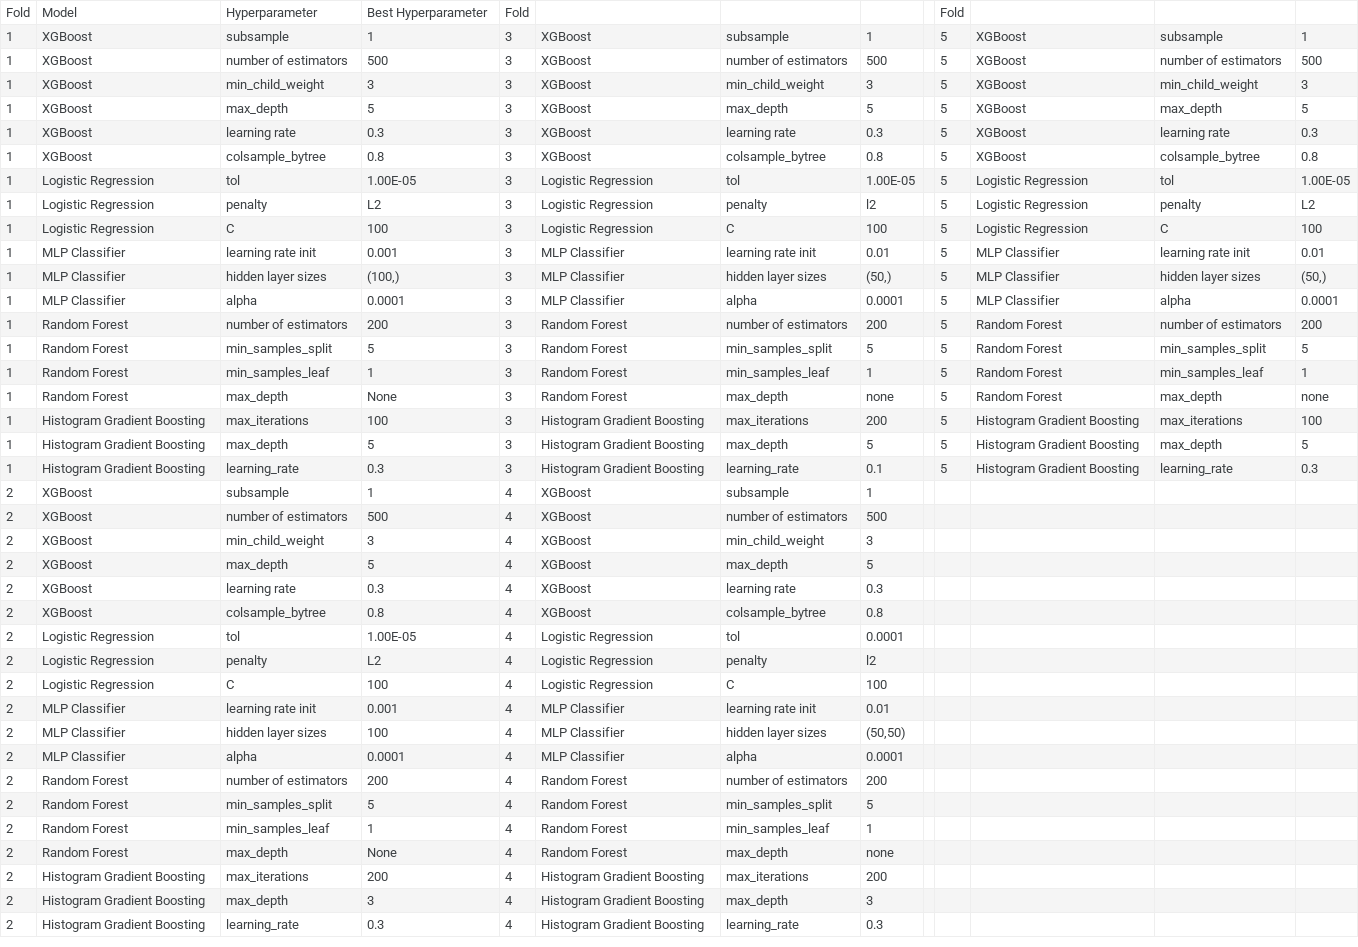
\includegraphics[scale = .35]{images/hyperparams.png}

\clearpage

\bibliographystyle{plainnat}
\bibliography{references}

\end{document}